\chapter{Independent Project in Information Engineering}

\section{Design thinking}
\begin{figure}[!ht]
    \centering
    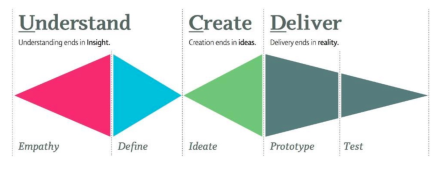
\includegraphics[width=10cm]{\imagesPath/design_thinking.png}
    \caption{The waterfall model. From~\cite{}} % DRIVHUSET slide 0
\end{figure}


\section{Innovation \& Immaterialrätt}
En bra affärside:
\begin{itemize}
\item \textbf{N}eed. Fråga de potentiella kunderna.
  \begin{itemize}
  \item Vad för problem har du upplevt?
  \item Beskriv den senaste gången du upplevde problemet?
  \item Hur ofta upplever du problemet?
  \item Hur brukar du lösa det?
  \item Hur skulle ditt liv bli bättre om problemet löstes?
    \item Hur mycket tid , pengar och energi kostar det dig?
  \end{itemize}
\item \textbf{A}pproach. Hur du designar lösningen.
\item \textbf{B}enefit. Du ska inte definera, värdet kunden gör det.
\item \textbf{C}ompetition. Google vad som finns.
\end{itemize}

\section{Källor och kritisk granskning}
Läs kritiskt
\begin{itemize}
\item Vad är det för typ av artikel?
\item Är det värt att läsa, vad kan artikeln bidra med?
\item Är den välskriven? (Begriplig, logisk, fakta/åsikter, referenser.
\end{itemize}
  
The five Cs
\begin{itemize}
\item Category
\item Context
\item Correctness
\item Contributions
\item Clarity
\end{itemize}

Läs effektivt

\textbf{Pass 1} (5 -10 min): Läs titeln, abstract, introduktion, rubriker, sammanfattning/conclusion och snapt kolla referenslistan. Utvärdera med Cs om det är värt att fortsätta.

\textbf{Pass 2} (max en timme): Läs artikeln men hoppa över svåra detaljer och antekna. Om det är värt att fortsätta gå till nästa pass.

\textbf{Pass 3} (fyra-fem timmar): Läs noggrant och fårstå allt.

Vetenskapligt skrivande:
\begin{itemize}
\item Precist och entydligt
\item Obektivt och neutralt
\item Sammanhängande
\item Uttömmande, ekonomiskt/effektivt
\item Klar och korrekt
\end{itemize}
  
%\textbf{Tips}
%\begin{itemize}
%\item If you tink about it, chanses are that somone else has as well. Therefore it is very important
%  that there is a stable foundation on projects that has not already beed done. If it has been done
%  but the project differs from the existing solutions, that is fine. But empfasise what the diffrence is.
%\item A reaseach project often draws knolage from several fealds. An example would be a project
%that looked at the application of artificial intelligence methods to predict breast cancer
%rates in patients – thus drawing together the two fields of medical science and artificial
%intelligence. 
%\item First define what are you looking for.
%\item \textit{relevance tree}, \textit{spider diagram} or \textit{research territory map} are good ways to find the realevance in the litreture you find useful in our prodject. 
%\end{itemize}
%
%
%- vi moste höja vår nivå, det är högre nivå i denna kursen
%åsikter ska inte varamed
%Kolla författaren
%Bra referenser.
%Ha flera omberoende referenser
%kolla regler system booken
%ta insperation för hur man skriver bra texter som man läser
%vi kommer läsa mer än 30 totalt
%
%IEEE should be use. BUt go for the mall. Dont just have number but try to understand it. Figure 3 is best to describe if it is on diffrent page. Dont have clickle text.
%
%Vi har relaterat arbete. Ett par sidor relaterat arbete.
%
%Man år andvända vi, blir lättare att läsa. Lätt läst är viktigt
%ej talspråk
%ej förtärknings språk
%objektiv (käller, ej åskikter)
%konsekvent stil svårt att ha flera,

\section{Crash-course inom dataskydd}
Historia i EU
\begin{itemize}
\item Rätten till Privacy (offentligrätt): art 7 EU stadgan
\item Rätten till Dataskydd (offentligrätt): art 8 EU stadgan
\item Dataskydd-GDPR (offentligrättslig som närmar sig till civilrätten)
\end{itemize}

GDPR handlar om personuppgifter som sparras och hanteras

Om personuppgifter ska behandlas på något sätt så måste följande motives.
\begin{itemize}
\item Nödvändighet att behanda datan
\item Andvändaren moste godkänna
\item Datan ska vara skyddad från andras åtkomst
\end{itemize}

Inbyggd dataskydd (DPbD)

Om man kan hellt anonymisera datan så behöver man inte tillämpa GDPR. Dock är detta vädigt svårt och är istället Pseudonymisera.

%usa (privacy)
%att ingen ska ta din data 
%
%eu (integretet)
%att datan ska haterat på ett bra och godkänt sätt
%
%gdpr 
%if personlig data
%if behandling (insamling också, digital)
%if registerande inom eu
%then gdpr
%
%if not lagrig grund
%eller not princisp
%    if ansvarige
%    
%behöver vi data
%balansera andvändaren och företaget
%
%anymisering du behandlar data därmef gdpr. sen behöver du inte tänka på det
%
%måste kunna bevisa att du har gjort det
%
%DPbD data protektion by design
%
%spara aldrig lösenord i klar text


\section{Etik}
God forskningssed
\url{https://www.vr.se/analys/rapporter/vara-rapporter/2017-08-29-god-forskningssed.html}

Klasisk filosofi
\begin{itemize}
\item Kants förnuftiga varelser
\item Mills lyckobegrepp
\item Aristoteles fronesis
\end{itemize}

sveriges ingenjörer hederskodex
``Ingenjören bör respektera anförtrodda upplysningars konfidentiella natur
samt andras rätt till uppslag, uppfinningar, utredningar, planer och ritningar.
Ingenjören får inte gynna obehöriga intressen och bör öppet redovisa
ekonomiska och andra intressen som kan påverka tilltron till hans eller hennes
opartiskhet och omdöme.
Ingenjören bör enskilt och offentligt, i tal och skrift, sträva efter ett sakligt
framställningssätt och undvika felaktiga, missvisande eller överdrivna påståenden.''
\url{https://www.sverigesingenjorer.se/om-forbundet/sveriges-ingenjorer/hederskodex/}


\section{Presentationsteknik}
En bra presentation:
\begin{itemize}
\item Anpassad till åhörarna
\item Bra ow, påläst, engagerat, humor
\item Inte innantill
\item Bra talteknik, artikulation, magstöd
\item Väl utformade slides
\item Alla involverade
\item Kroppspråk
\item Tydligt budskap
\end{itemize}
% 09 Presentationsteknik 8

Det man tar upp:
\begin{itemize}
\item Motivationen först!
\item Det viktigaste först, sen successivt mindre viktiga saker.
\item Vad har ni gjort och hur, och varför? Hur gick det?
\item Använd exempel!
\end{itemize}

Vad man inte tar med:
\begin{itemize}
\item Live-demo (men inspelad är ok)
\item Referenslistan med relaterat arbete
\item Vad man inte hann
\item Alla detaljer
\end{itemize}

Exempel på upplägg:
\begin{itemize}
\item Motivera åhörarna, väck intresse
\item Beskriv problemet/problemställningen, varför det är viktigt
\item Vad har ni gjort/byggt/åstadkommit?
\item Hur gjorde ni? (men inte alla detaljer!)
\item Vad blev resultatet, hur bra?
\item Sammanfattning
\end{itemize}

Kontakt och nerver:
\begin{itemize}
\item Läs inte innan men det kan vara bra att ha manus eller stödord som stöd. Man kan också bara ha den första meningen.
\item Ha ögonkontakt och le lite. Att le hjälper med nerverna.
\item Andvänd kroppspråk. 
\item Öva mycket och när du övar gör gärna framför andra eller bara prata för dig skjälv.
\item Prata långsamt, andas, drik vatten.
\end{itemize}

Bra slides:
\begin{itemize}
\item Bilder och ilustrationer för ren text.
\item Bra att ha text också men inte för mycket åt en gång.
\item Fake punkt listor.
  \item Det kan vara svårt att se text i slides om man sitter långt borta.
\end{itemize}



% \section{Pattent}
%självstudie kurs kolla studium.
%
%Namnet får inte referera till produktern
%
%25år design kyd geographismkt
%
%upphovsrätt R namn år
%
%håll hemligt innan patent annars får man inte det
%
%teknat, avtal
%
%\section{df}
%små steg energi intense
%
%dont have alwae running
%
%we should use mål as a refrence, this is realy imortant even fn says it is
%
%make disition based on mål
%
%färg blind
%
%kolla på vad som tar energi
%
%development hålbarhat
%readability
%
%\section{c}
%
%backrund läg fokus
%
%innan man har fåt granskad kan man publicera på denna sidan https://arxiv.org/
%
%Kolla på wikipedia för primär källor
%
%\url{https://libguides.ub.uu.se/}  får bra resurcer
%kola tidskrifter för att kolla peer review
